\chapter{System Design}
\label{chp:design}

How to measure swarm by looking at Swarm evolution \cite{2013:swarmevolution:su}.
Helper in swarm without need of human intervention \cite{2014:bwmarket:capota}. Aligning supply and demand of bandwidth

\section{Credit Mining Main Components}

\begin{itemize}
\item general flow
\item similarity check
\end{itemize}


\begin{figure}[ht]
	\centering
	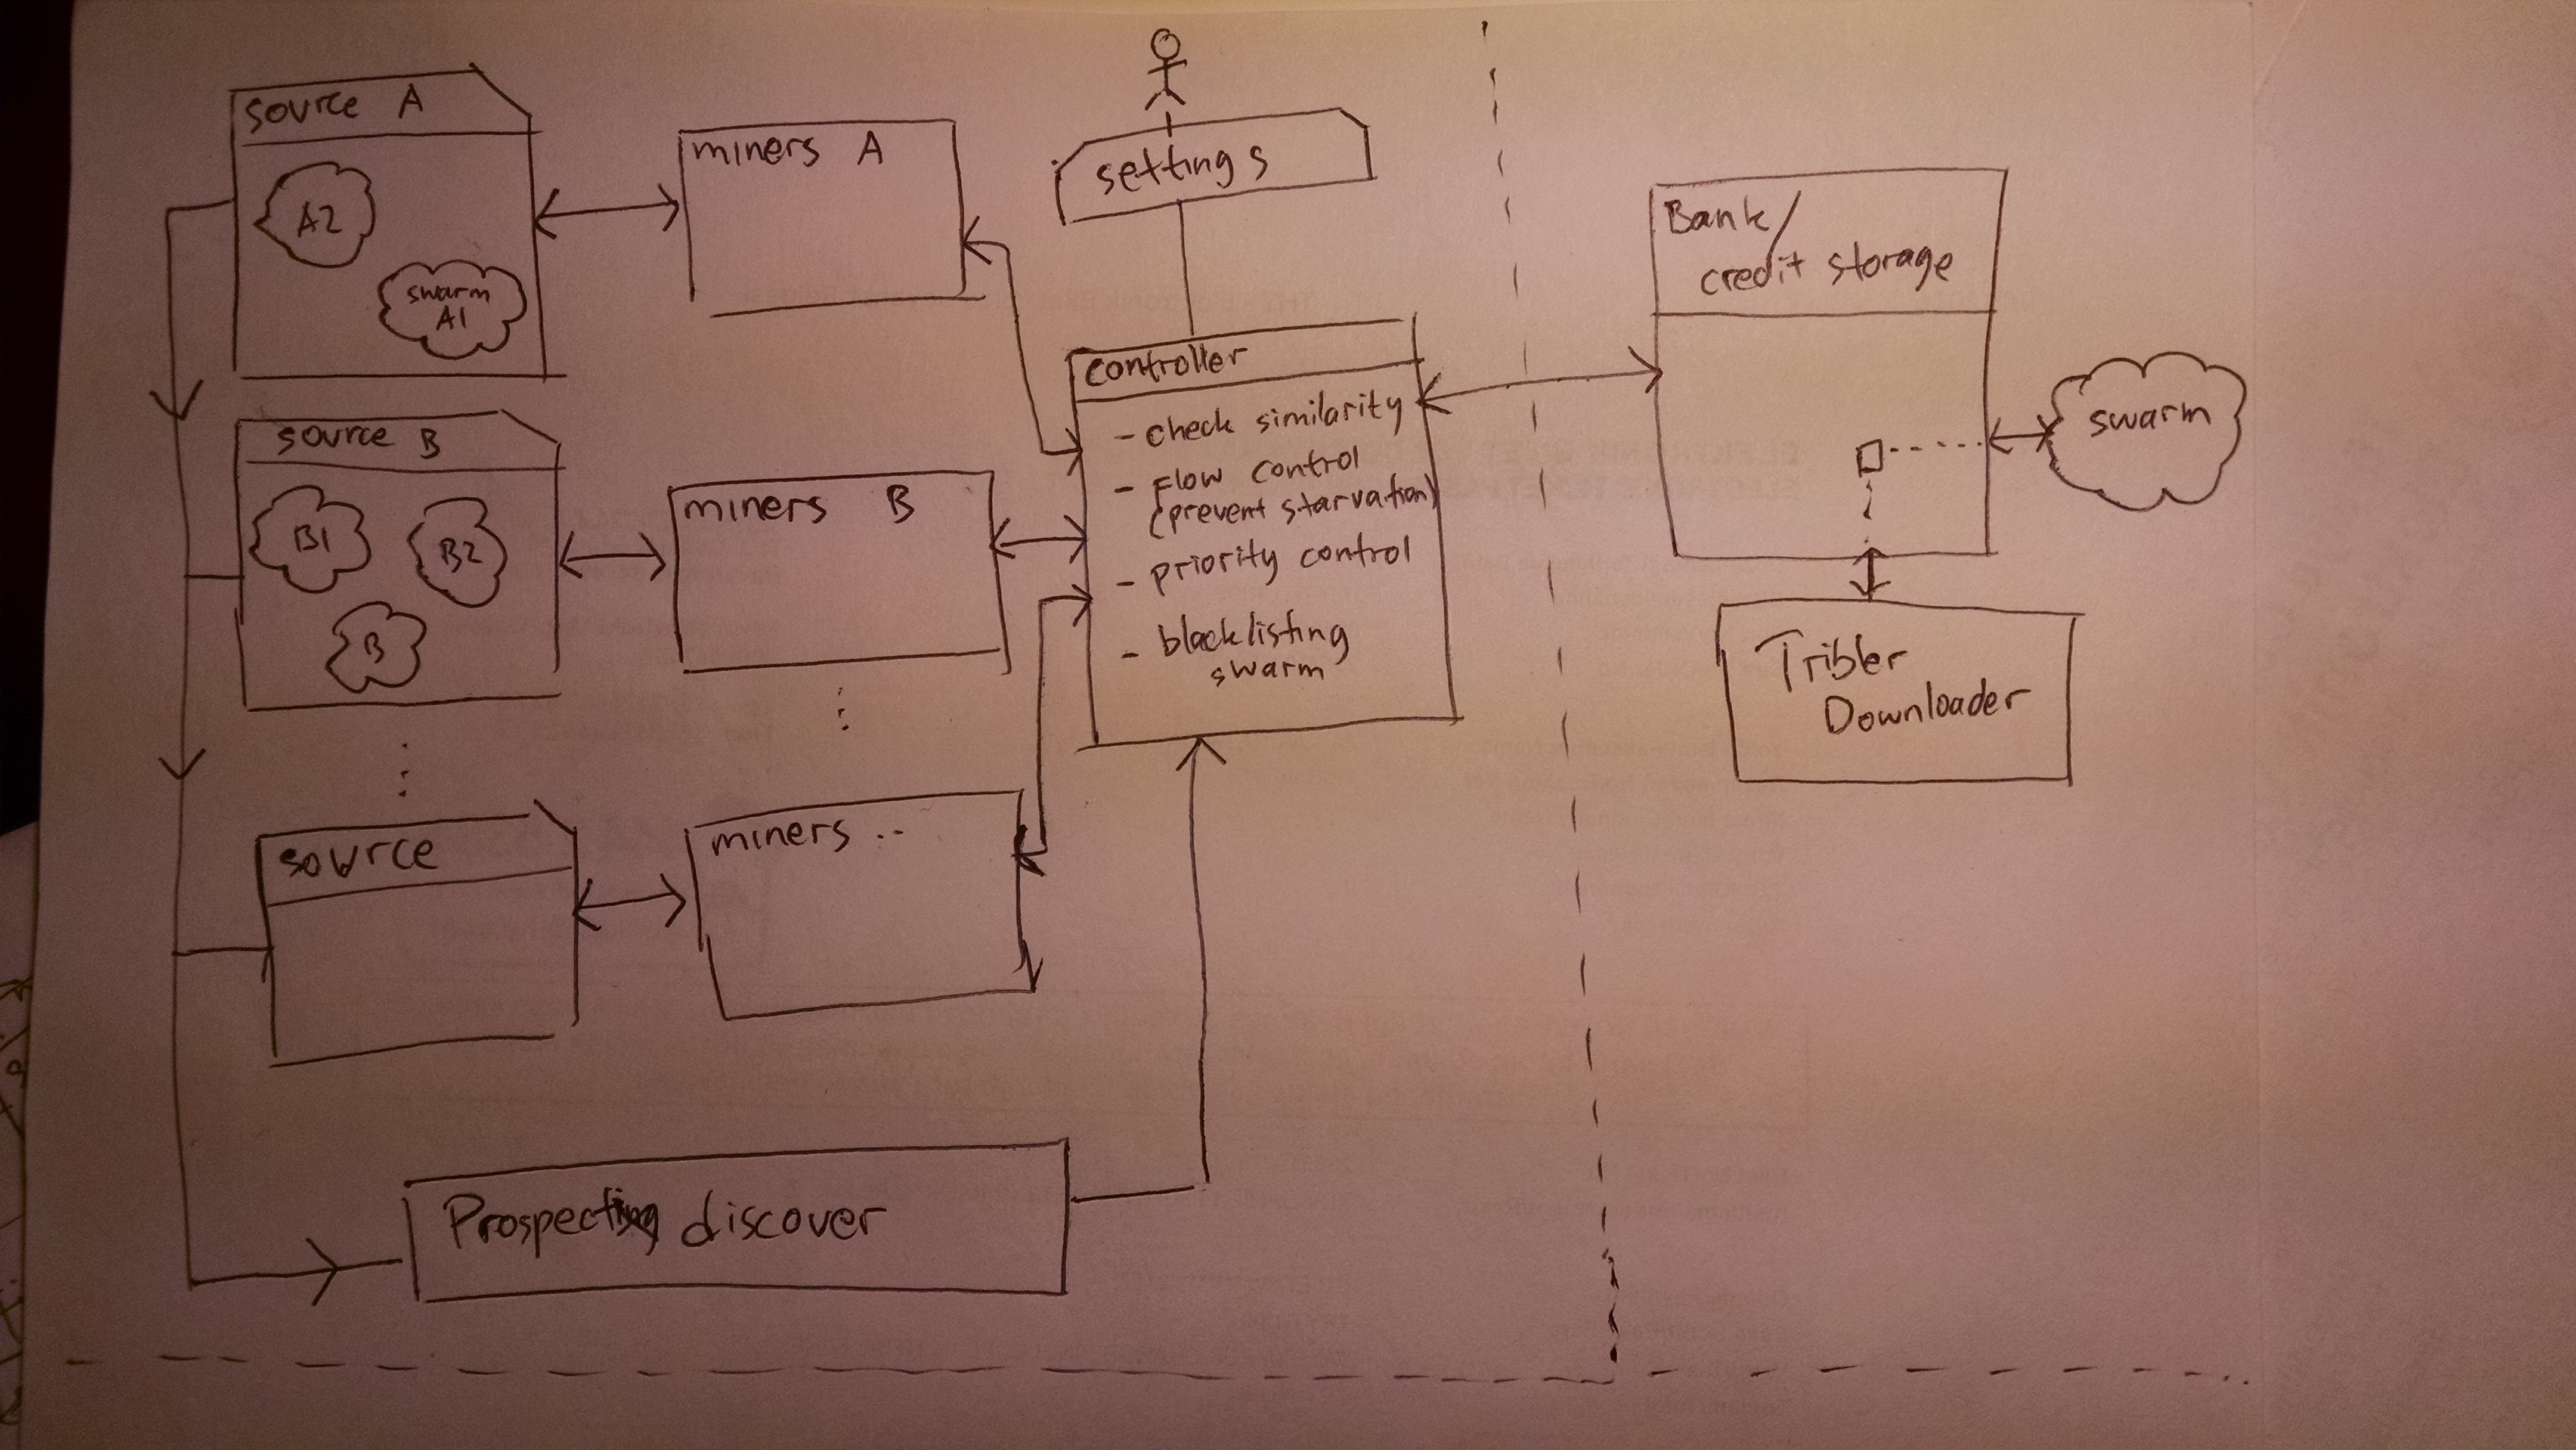
\includegraphics[width=\textwidth]{pics/cm_components.jpg}
	\caption{TEMP:Credit mining components.}
	\label{fig:cmcomponents}
\end{figure}

\subsection{Mining Sources}
\begin{enumerate}
	\item rss
	\item channel
	\item directory source
\end{enumerate}

\subsection{Swarm Selection}
 policies : 
\begin{enumerate}
	\item random
	\item swarm age
	\item seeder ratio
\end{enumerate}

\subsection{Prospecting Methodology}
prospect a swarm : 
\begin{enumerate}
	\item N-piece
	\item peer translation (peer info to swarm info)
\end{enumerate}

\subsection{Resource Optimization}
\begin{itemize}
	\item starvation prevention, no immediate stopping
	 \item fallback mechanism (for now)
\item 	 swarm blacklisting
\item 	 resume downloading (cache)
\item 	 archival mode
\end{itemize}


\section{Tribler integration}
Tribler is well known for its anonymity and secure interface on top of \bt~ network. In 2014, Tribler published a specification on its anonymity feature\footnote{\url{https://github.com/Tribler/tribler/wiki/Anonymous-Downloading-and-Streaming-specifications}}. It uses Tor-like onion routing with purely distributed mechanism. A year later, \citeauthor{2015:tunnel:ruigrok} on his work completed the \textit{tunnel community} which emphasize end-to-end encryption in Tribler. This comes with several drawbacks. The most important one is performance degradation. Adding layers of privacy comes with increasing the amount of cryptography operation which slows down end-to-end downloading activity \cite{2015:tunnel:ruigrok}.

\subsection{Experience enhancement}
\begin{itemize}
\item  aware user download, priority mehcnism
\item  enable/disable relaxation
\item single click choose channel
\end{itemize}

\subsection{Anonymous and secure mining}
\begin{itemize}
\item  usage of tunnel community
\item  multichain?
\end{itemize}

\section{Libtorrent}
Another Tribler dependency is \textit{libtorrent}\footnote{\url{http://libtorrent.org/}}. With \bt~is just a collection of specification, it free to be implemented with any languages. One of the implementation in \texttt{C++} is \textit{libtorrent}. \textit{libtorrent} also has \texttt{python} binding which the same language as Tribler implementation. \textit{Libtorrent} started in 2003 by Arvid Norberg. \textit{Libtorrent} is used by many torrent client such as Deluge, qBittorrent, Free download managers, and many others.

\subsection{Priority Management}
priority in libtorrent. Unchoke round. Bandwidth control

\subsection{Share Mode}
One of the crucial feature used in this work is \textit{share mode} \footnote{Core code of share mode can be found in \url{https://github.com/arvidn/libtorrent/blob/master/src/torrent.cpp\#L9586-L9727}}. Initial work performed by \citeauthor{2015:creditmining:capota} also used this feature\cite{2015:creditmining:capota}. By enabling share mode, it means that one is not interested in downloading the file, but gaining higher share ratio. It is done by download as little as possible and upload as much as possible. Share mode only download a torrent where it has sufficient capacity. A torrent downloaded in share mode may never finish as \textit{libtorrent} only download piece of a torrent which satisfied the share mode requirements. Share mode can be enabled per torrent basis.

Share mode algorithm works heuristically as it estimates the rarest piece available in the swarm based on participated peers. First, it tries to find whether there is a piece which nobody has (line \ref{alg:l_lts:missingp}). Note that in line \ref{alg:l_lts:disconnectpeers}, libtorrent disconnect some of the seeder because we need to connect to the leecher later. This case is considered if there are too many seeder in our connection pool. Next, the number of missing pieces is decreased linearly with the number of seeder. This is based on assumption that both of us and other seeder can upload at least one piece each (line \ref{alg:l_lts:reducemissing}). To keep the performance, downloading piece activity is stacked until more than 5\% of the number to be downloaded (line \ref{alg:l_lts:retdling}). To determine rarest piece, libtorrent count the number of peer that has that piece. The number of peer on the rarest piece is termed \textit{rarity}. Share mode ensure that we only download the rarest piece available in the network (line \ref{alg:l_lts:rarepc}). We end the prematurely routine if there are more number of piece to download compared to uploaded (line \ref{alg:l_lts:retdlenough}) or there are not enough peer to upload the rarest piece (line \ref{alg:l_lts:rareunable}). Both condition will prevent us to get positive share ratio. Finally, it will download randomly the rarest pieces if there are more than one option (line \ref{alg:l_lts:dlrare}). The algorithm presented in algorithm \ref{alg:ltsharemode}. 

\begin{algorithm}[]
	\caption{Libtorrent share mode algorithm}
	\label{alg:ltsharemode}
	\begin{algorithmic}[1]
		\Require{$T$ as share mode target}
		\Statex
		\State{$missing\_piece = 0$}
		\ForAll{$p \in connected\_peers$}
		\If{$p$ is a $leecher$ $and$ $p$ is not in share\_mode}	
		\State{$missing\_pieces$} += {$total\_pieces - pieces(p)$} \label{alg:l_lts:missingp}
		\EndIf	
		\EndFor
		\If{$|connected\_seeders|$ in $connected\_peer$ $>$ $90\%$}	
		\State disconnect excess seeder \label{alg:l_lts:disconnectpeers}
		\EndIf
		\State{$missing\_pieces$} -= {$2 \times |connected\_seeders|$}	\label{alg:l_lts:reducemissing}	
		\If{$missing\_pieces \leq 0$}
		\State \Return
		\EndIf
		\If{$num\_to\_downloaded \times T > uploaded$} \label{alg:l_lts:retdlenough}
		\State \Return
		\EndIf
		\If{$downloading < 5\% \times num\_to\_downloaded$} \label{alg:l_lts:retdling}
		\State \Return
		\EndIf
		\ForAll{$pc \in pieces()$}
		\If{$pc$ not in $collected\_piece$ $and$ $peer\_count(pc) \leq rarest\_rarity$ }	\label{alg:l_lts:rarepc}
		\State{$rarest\_rarity$} = {$peer\_count(pc)$} 
		\State{$rare\_piece$.push($pc$)}
		\EndIf	
		\EndFor
		\If{$|connected\_peers| - rarest\_rarity < T$} \label{alg:l_lts:rareunable}
		\State \Return
		\EndIf
		\State download {$random(rare\_piece)$} \label{alg:l_lts:dlrare}
	\end{algorithmic}
\end{algorithm}

There are several limitations on this feature as we observed. First, it only has single parameter which determine the desired target of share ratio. This limits the exploration and full use of share mode feature. Another issues are storage and network inefficiency. If enabled, share mode works by downloading popular piece of a particular torrent. This means few downloaded pieces could take a large storage. Share mode also did not check whether a swarm is efficient enough to perform this operation. It only tries to find popular pieces regardless of the swarm condition. It is highly possible that if a swarm is in poor capacity, the uploading rate is very low. The bandwidth used to check torrent pieces regularly is wasted and the ``investment'' will not go well.